\chapter{Binære Træer}
\label{ch:Binære Træer}


\section{Hvad er et Træ}
\label{sec:Hvad er et Træ}

Træer som vi kender dem, har en stamme hvorfra grene springer ud. Fra grenene springer mindre grene, og på den måde ender træet med at have mange små grene, som stammer fra samme stamme. Informatikkens træer er ikke langt fra denne forståelse. I informatik er træer en datastruktur. Det er et netværk af knudepunkter forbundet af kanter. Træet starter med roden, der typisk er tegnet øverst (se figur \ref{fig:Eksempel på træ.}). En rod er hvor træet begynder, og har ingen forældre. Fra roden forgrener træet sig til flere, børn der også kan have flere børn. Træstrukturen er sådan at man altid kan vælge et knudepunkt, og lave et subtræ med kudepunktet som rod. Knudepunkterne hvor træet ender kalder man blade. Informatikkens træer har også en dybde. Hvis man starter ved roden, er dybden $0$. Hver gang man går et trin "ned", i træstrukturen, stiger dybden med $1$. Det betyder at den maksimale dybde svarer til træets højde. \cite{trees}


\section{Et Binært Træ}
\label{sec:Et Binært Træ}

Man tegner normalt binære træer som på figur \ref{fig:Eksempel på binært træ} bestående af knudepunkter og forbindelser mellem dem. Det specielle ved \emph{binære} træer, er at hvert knudepunkt højst må forgrene sig to gange (altså binært). Denne lille specialisering er brugbar i mange sammenhænge som f.eks. som datastruktur til søgealgoritmer \cite{BST}, men det viser sig også at være en snedig vej til at beskrive sorteringsalgoritmers opførsel.

\begin{figure}
	\begin{center}
		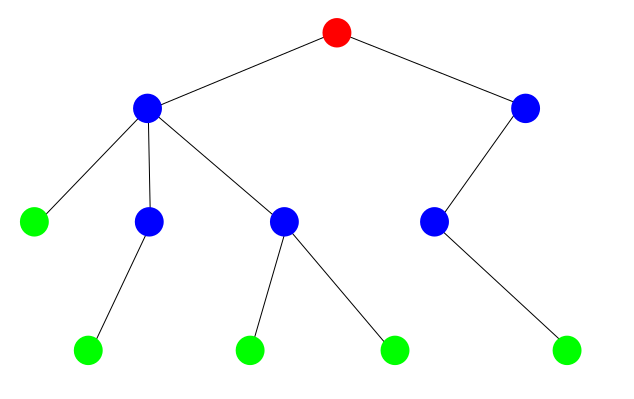
\includegraphics[scale=0.35]{../img/tree.png}
	\end{center}
	\caption{Eksempel på træ.}
	\label{fig:Eksempel på træ.}
\end{figure}



\begin{figure}
	\begin{center}
		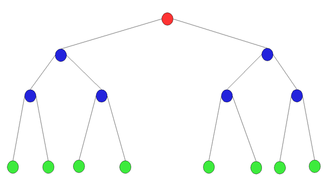
\includegraphics[scale=1]{../img/binary_tree.png}
	\end{center}
	\caption{Eksempel på binært træ. Træets balde er markeret med \green{grøn}, og roden med \red{rød}. \cite{binaert-trae}}
	\label{fig:Eksempel på binært træ}
\end{figure} 


\section{Blade i et Fuldt Binært Træ}
\label{sec:Blade i et Fuldt Binært Træ}

Beviset er baseret på kilden \cite{tree-leaves}.\\

Et fuldt binært træ, er et binært træ, hvor alle bladene har samme dybde. Træet på figur \ref{fig:Eksempel på binært træ}, er et fuldt binært træ. \\

Intuitivt giver det mening, at hvert knudepunkt har to børn, og at antallet af blade derfor er givet ved $2^d$, hvor $d$ er træets dybde. Dette udtryk kan bevises således:\\

Vi antager at et træ med en maksimal dybde $d$, har $2^d$ blade.\\

Hvis vores dybde er $d + 1$, skal antallet af blade være $2^{d+1}$.\\

I et fuldt binært træ fordobles antallet af blade, hver gang dybden stiger med $1$. Det er fordi alle knudepunkter i et fuldt binært tre, altid forgrener sig til to børn. Altså må antallet af blade ved dybden $d+1$, være det dobbelte af antallet af blade ved dybden $d$.

$$2\cdot (2^d)$$

Vi kan nu omskrive udtrykket således:

$$2\cdot (2^d) \,\,\,=\,\,\, 2^1 \cdot 2^d \,\,\,=\,\,\ 2^{d+1}$$

Altså er antagelsen, at antallet af blade i et fuldt binært træ er $2^d$, bekræftet. $\blacksquare$\\

Det er vigtigt at pointere at alle binære træer med dybden $d$, maksimalt har lige så mange blade, som det fulde træ med samme dybde. Altså er $2^d$ også det maksimale antal blade for er generelt binært træ, med dybden $d$.



\section{Binære Træer og Sorteringsalgoritmer}
\label{sec:Binære Træer og Sorteringsalgoritmer}

Ved første blik kunne man tilgives for ikke, at se hvordan binære træer har relevans for sorteringsalgoritmer, men det kræver bare, at man giver knudepunkterne og grenene meningsfulde betydninger. I bund og grund er det som en sorteringsalgoritme gør, at fortage en masse sammenligninger af elementerne i dens input. Algoritmen bestemmer hvilke operationer, den skal køre udelukkede på baggrund af disse sammenligninger. Hvis vi tænker hvert knudepunkt som en sammenligning af to elementer fra algoritmens input (se figur \ref{fig:Binært Træ for Sammenligninger}), er det jo givet, at det ene element enten vil være større end det andet eller ikke større. Denne sammenligning guider algoritmens operationer og derved den næste sammenligning. Dette gentages til algoritmen har gjort nok sammenligninger, til at kunne sortere dens input. Vi kan derfor tænke alle træets blade, som en måde for algoritmen at sortere et bestemt input; Hvert blad har kun en specifik vej, og vejen til bladet er udelukkede givet af algoritmens input. Altså er hvert af træets blade en kollektion af de sammenligninger, som algoritmen gjorde for at sortere inputtet. \cite[s. 109]{aogd}

\subsection{Det Mindste antal Sammenligninger}%
\label{sub:Det Mindste antal Sammenligninger}

I dette store teoretiske træ med alle dets blade kunne man jo så spørge: Hvor mange sammenligninger skal der så højest til at sortere et input? eller omformuleret: Hvor højt er træet? Denne oversættelse holder stik, da vi skal lave lige så mange sammenligninger for at komme ned til nederste blad, som træet er højt.

\begin{figure}
	\begin{center}
		\begin{tikzpicture}[scale = 1.5]
			\tikzstyle{comp} = [rectangle, draw, rounded corners];
			\node (12) at (0,0) {$e_1 \:?\: e_2$};
			\node (23) at (-3,-1)  {$e_2 \:?\: e_3$};
			\node (23b) at (3,-1)  {$e_2 \:?\: e_3$};
			\node (13) at (-2,-2)  {$e_1 \:?\: e_3$};
			\node (13b) at (2,-2)  {$e_1 \:?\: e_3$};
			\node (ww) at (-4,-2) {$e_1\leq e_2\leq e_3$};
			\node (1w3s2) at (-3,-3) {$e_1\leq e_3< e_3$};
			\node (3s1w2) at (-1,-3) {$e_3< e_1\leq e_2$};
			\node (2s1w3) at (1,-3) {$e_2< e_1\leq e_3$};
			\node (2w3s1) at (3,-3) {$e_2\leq e_3< e_1$};
			\node (1g2g3) at (4,-2) {$e_1> e_2> e_3$};
			\draw [->] (12) to node [above] {$\leq$} (23);
			\draw [->] (23) to node [above] {$\leq$} (ww);
			\draw [->] (12) to node [above] {$>$} (23b);
			\draw [->] (23) to node [above] {$>$} (13);
			\draw [->] (13) to node [above] {$\leq$} (1w3s2);
			\draw [->] (13) to node [above] {$>$} (3s1w2);
			\draw [->] (13b) to node [above] {$\leq$} (2s1w3);
			\draw [->] (13b) to node [above] {$>$} (2w3s1);
			\draw [->] (23b) to node [above] {$\leq$} (13b);
			\draw [->] (23b) to node [above] {$>$} (1g2g3);
		\end{tikzpicture}
	\end{center}
	\caption{Binært Træ. \cite[s. 109]{aogd}}
	\label{fig:Binært Træ for Sammenligninger}
\end{figure}

\section{Højden af et Binært Træ}
\label{sec:Højden af et Binært Træ}

Dette bevis er basseret på kilden \cite[s. 109]{aogd}.\\


\emph{Bevis:} I et sammenligningstræ for en sorteringsalgoritme med input længden $n$, hvor $\pi$ og $\sigma$ er permutationer af listen $\{1 \dots n\}$, er bladene der svarer til $\pi$ og $\sigma$ ($l_{\pi}$ og $l_{\sigma}$) forskellige.\\

Dette er et modstridsbevis hvilket betyder, at vi starter med at antage det modsatte, af det vi prøver at bevise: vi antager altså at $\pi$ og $\sigma$, leder til samme blad i sammenligningstræet; $l_{\pi}$ og $l_{\sigma}$ er ens.\\

Under denne antagelse kan to forskellige lister $\{e_1 \dots e_n\}$ og $\{e_1' \dots e_n'\}$, gennemgå de \emph{præcis} samme operationer og derved sortere listen. Dette er en modstrid, da man aldrig vil kunne benytte præcis de samme operationer, til at sortere to forskellige permutationer af $\{1 \dots n\}$. $\blacksquare$ \\


Alle permutationer af listen $\{1 \dots n\}$ har altså et tilsvarende blad, derfor må sammenligningstræet have mindst $n!$, da der skal være et for hver permutation.\\

Det maksimale antal blade på et binært træ er $2^d$, hvor $d$ er træets dybde (som vi beviste i afsnit \ref{sec:Blade i et Fuldt Binært Træ}). Vi kan nu opstille denne ligning:


$$2^d \geq n! \s\Leftrightarrow\s d \geq \log n!$$

For at bygge videre kan vi nu bruge regnereglen $n! \geq \left( \frac{n}{e} \right)^n$

$$d \geq \log n! \geq \log \left(\left(\frac{n}{e}\right)^n\right)$$

Ved hjælp af logaritmeregneregler kan vi omskrive udtrykket længst til højre således:

$$\log \left(\left(\frac{n}{e}\right)^n\right) = n \cdot \log \left(\frac{n}{e} \right) = n \cdot \log n - n \cdot \log e$$

Dette er altså et udtryk for højden af et sammenligningstræ:

$$d \geq n \cdot \log n - n \cdot \log e$$

Da $d$ er træets dybde, er det også det maksimale antal sammenligninger en given sorteringalgoritme skal gøre, for at sortere en liste. Udtrykket siger at den nedre grænse for $d$ er $n \cdot \log n - n \cdot \log e$. Det er altså ikke muligt at sortere en liste med færre sammenligninger i værste tilfælde. Da antallet af sammenligninger er proportionalt med algoritmens udførelsestid, må det være sandt at alle sorteringsalgoritmer har en nedre værste-tilfælde-vækstrategrænse på $O(n \cdot \log n)$.


\section{Store-O er Værste Tilfælde}
\label{sec:Store-O er Værste Tilfælde}

Det er en vigtigt detalje, at denne nedre grænse er for vækstraten i \emph{værste} tilfælde. Insertionsort kan i bedste tilfælde sortere en liste med $O(n)$ \cite{big-o-cheatsheet}, men det er værste tilfælde som vækstraten-gænsen gælder for. Det er muligt at sortere en liste hurtigere end $O(n \cdot \log n)$, det kræver bare at det ikke er det værste tilfælde, og at algoritmen (som insertionsort) kan sortere listen hurtigere i bedste tilfælde. Man burde hellere tænke grænsen således: Man kan aldrig lave en sorteringalgoritme, der virker ved hjælp af sammenligninger, som vi kan være sikrer på, er hurtigere end $O(n \cdot \log n)$.

\section{Mergesort og Den Nedre Grænse}
\label{sec:Mergesort og Den Nedre Grænse}

Vi ved nu at alle sorteringsalgoritmers værste-tilfælde-vækstrate, er afgrænset af $O(n \cdot \log n)$. Vi ved også at mergesort har tidskompleksiteten $O (n \cdot \log n)$. Mergesort har altså den teoretisk bedste tidskompleksitet for en sammenlignings-sortering-algoritme. Ikke nok med det betyder det også at mergesort både i bedste og væreste tilfælde er $O(n \cdot \log n)$. Mergesort er altså $\Theta (n \cdot \log n)$.


$$T_{\text{mergesort}}(n) \,\,\in\,\, \Theta (n \cdot \log n)$$




%Binære træers højde måles på hvor mange forgreninger, skal til for at nå det yderste blad.


